\documentclass[a4paper]{report}
\usepackage{Rnews}
\usepackage[round]{natbib}
\usepackage{array}
\usepackage{graphicx}
\bibliographystyle{abbrvnat}

\begin{document}

\begin{article}
\author{by Nitin Jain and Gregory R. Warnes}
\title{Balloon Plot}
\subtitle{Graphical tool for displaying tabular data}

\maketitle

\section*{Introduction}

Numeric data is often summarized using rectangular tables. While
these tables allow presentation of all of the relevant data, they do
not lend themselves to rapid discovery of important patterns. The
primary difficulty is that the visual impact of numeric values is
not proportional to the scale of the numbers represented.

We have developed a new graphical tool, the \code{balloonplot},
which augments the numeric values in tables with colored circles
with area proportional to the size of the corresponding table
entry. This visually highlights the prominent features of
data, while preserving the details conveyed by the numeric values
themselves.

In this article, we describe the balloonplot, as
implemented by the \code{balloonplot} function in the
\code{gplots} package, and describe the features of our
implemenation.


\section*{Function description}

The \code{balloonplot} function accepts a table (to be displayed as
found) or a vector or list of vectors for x (column category), y
(row category) and z (data value) of vectors from which a table will
be constructed.  

The \code{balloonplot} function plots a graphical table,
where each cell displays the appropriate numeric value plus a
colored circle whose size reflects the relative magnitude of the
corresponding component. The
\emph{area} of each circle is proportional to the frequency of
data. (The circles are scaled so that the circle for largest value
fills the available space in the cell.)


As a consequence, the largest values in the table are ``spotlighted''
by the biggest cicles, while the smaller values are displayed
with very small circles.  Of course, circles can only have positive
radius, so the radius of circles for cells with negative values are
set to zero.  (A warning is issued when this ``truncation'' occurs.)

Of course, when labels are present on the table or provided to the
function, the graphical table is appropriately labeled.  In
addition, options are provided to allow control of various visual features
of the plot:

\begin{itemize}
  \item rotation of the row and column headers
  \item balloon color and shape (globally or individually)
  \item number of displayed digits
  \item display of entries with zero values
  \item display of marginal totals
  \item display cumulative histograms
  \item x- and y-axes group sorting
  \item formatting of row and column labels
  \item as well as the traditional graphics parameters (title,
    background, etc.)
\end{itemize}

\section*{Example using the \code{Titanic} data set}

For illustration purposes, we use the \code{Titanic} data set from
the \code{datasets} package.  \code{Titanic} provides survival status
for passengers on the tragic maiden voyage of the ocean liner
``Titanic'', summarized according to economic status (class), sex, and
age.


%Using \code{balloonplot}, we display the number of people surviving
%the Titanic tragedy, - figure~\ref{figure:Surv.Pop} categorized by gender, age
%and class.  Total number of people on
%Titanic are displayed in figure~\ref{figure:Total.Pop}. Finally, the
%proportion of surviors is shown in figure~\ref{figure:Surv.Pop}.


%%
%%\begin{table}[!ht]
%%\begin{center}
%%\begin{tabular}{rrrrr}
%%\hline
%% & Child-M & Child-F & Adult-M & Adult-F \\
%%\hline
%%1st & 5.00 & 1.00 & 57.00 & 140.00 \\
%%2nd & 11.00 & 13.00 & 14.00 & 80.00 \\
%%3rd & 13.00 & 14.00 & 75.00 & 76.00 \\
%%Crew & 0.00 & 0.00 & 192.00 & 20.00 \\
%%\hline
%%\end{tabular}
%%\end{center}
%%\end{table}
%%
%%

%%\begin{figure}
%%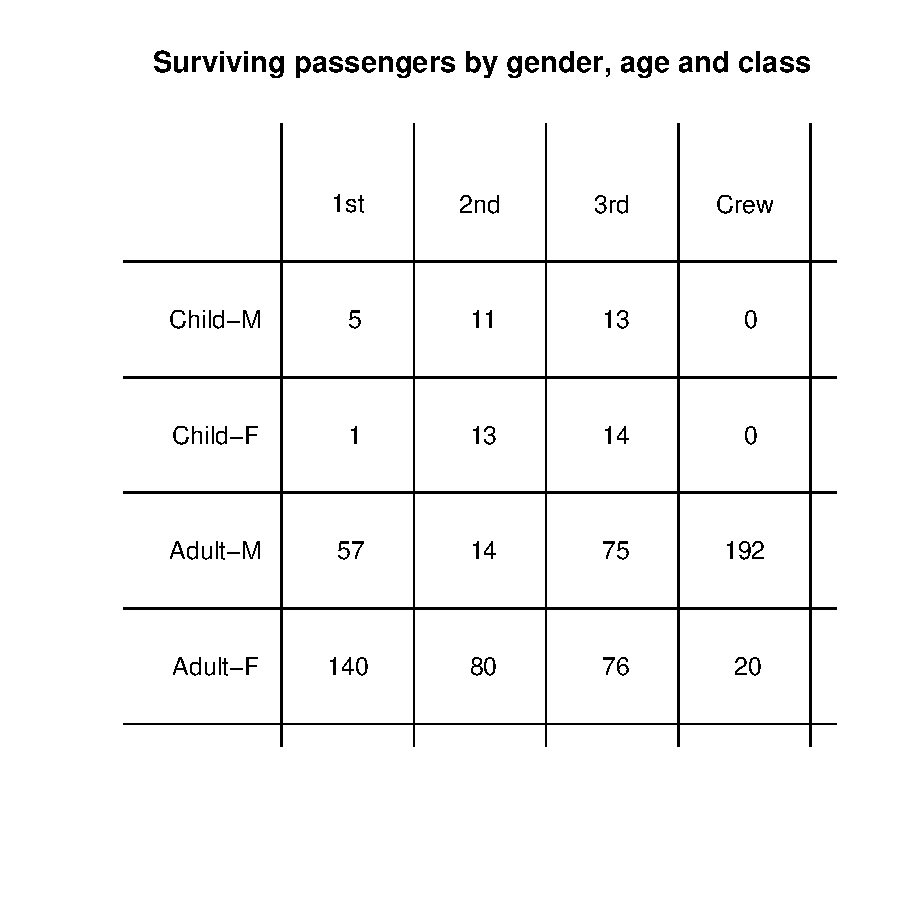
\includegraphics[width=\textwidth]{SurvivedPopWhite.pdf}
%%\vspace*{-0.25in}
%%\caption{\label{figure:Surv.Pop.White}
%%Tabular representation of surviving population}
%%\end{figure}
%%
%%
%%Figure~\ref{figure:Surv.Pop.White} displays a graphical table
%%without balloons.  (This was created by calling balloonplot with
%%the balloon color set to match the background color.)  Note
%%that one must explicitly pay attention to the values in the cells in
%%order to see any pattern in the data.
%%


Typically, the number of surviving passengers are shown in a tabular
form, such as shown in Figure~\ref{figure:Table}.  (This was created
by calling balloonplot with the balloon color set to match the
background color.)  Note that one must actively focus on the
individual cell values in order to see any pattern in the data.

\begin{figure}
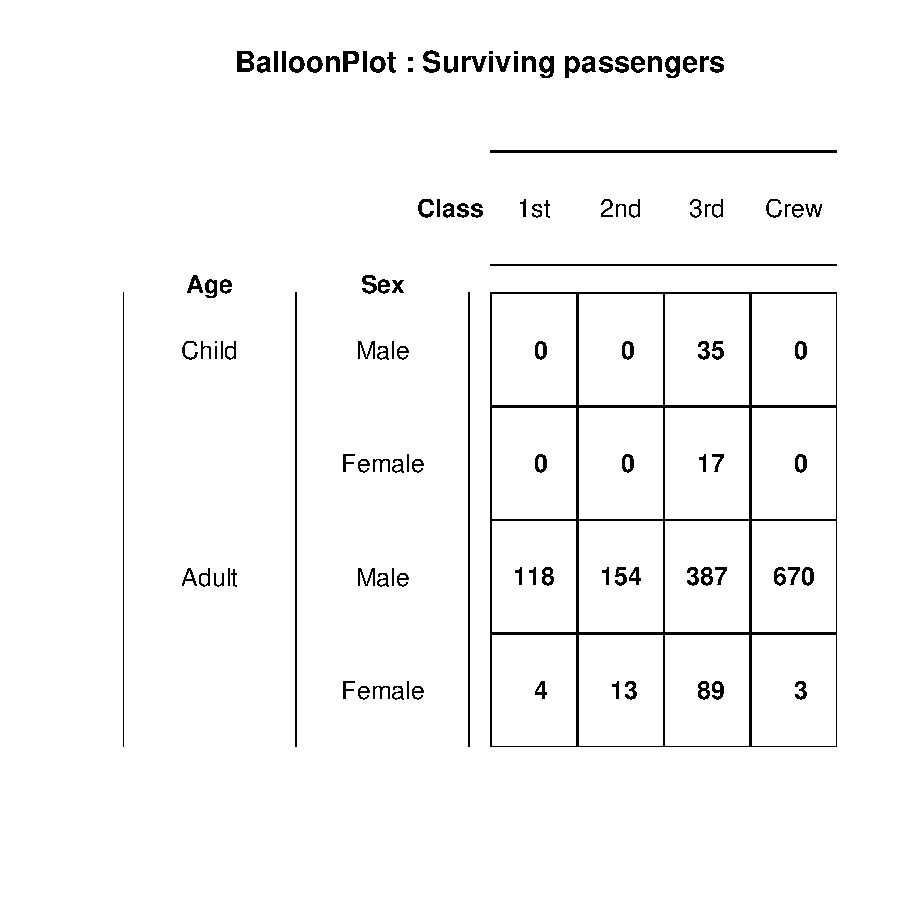
\includegraphics[width=\textwidth]{Figure1.pdf}
\caption{\label{figure:Figure1}
Tabular representation of survived population by gender and age}
\end{figure}


Now, we redraw the table with light-blue circles (`balloons')
superimposed over the numerical values
(figure~\ref{figure:Figure2}).  This is accomplished using the code:

{\small
\begin{verbatim}
library(gplots)
library(datasets)

data(Titanic)

dframe <- as.data.frame(Titanic)
 ## convert to 1 entry per row format

survived <- dframe[dframe$Survived=="No",]
attach(survived)

balloonplot(x=Class, y=list(Age, Sex), z=Freq,
            sort=TRUE, show.zeros=TRUE,
            cum.margins=FALSE, main=
            "BalloonPlot : Surviving passengers")
mtext("by class, gender, and age")

detach(survived)
\end{verbatim}
}
%$

\begin{figure}
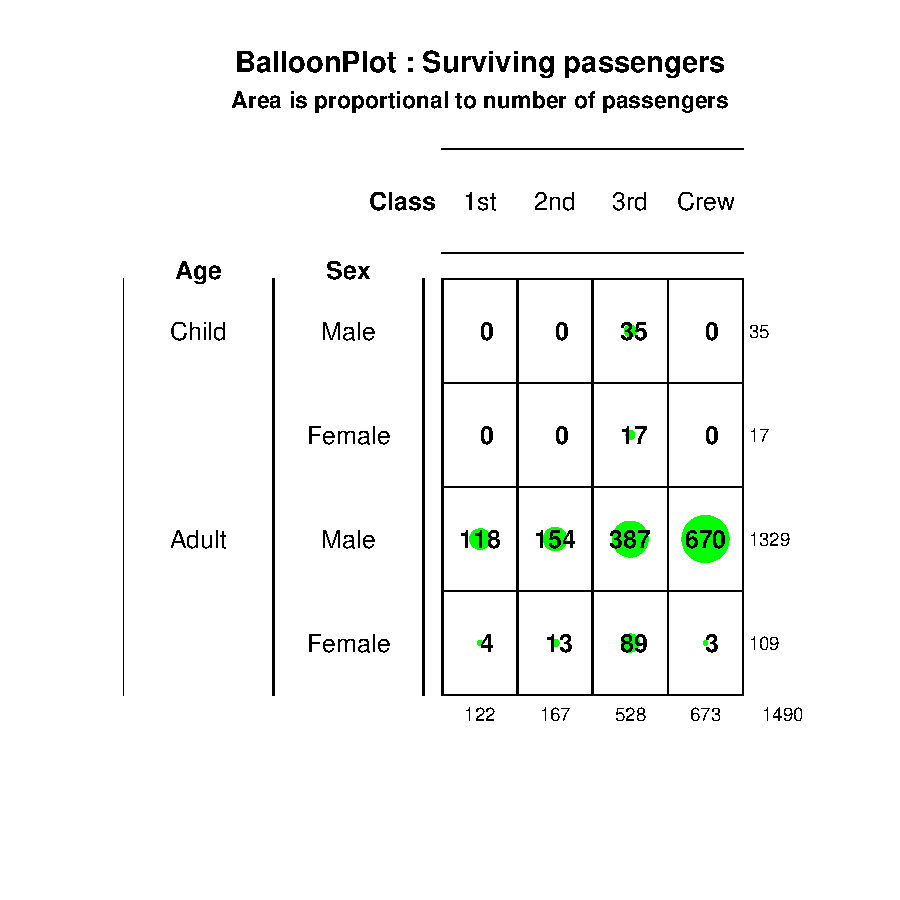
\includegraphics[width=\textwidth]{Figure2.pdf}
\caption{\label{figure:Figure2}
Balloon plot of surviving individuals by class, gender and age }
\end{figure}

With the addition of the blue ``spotlights'', whose area is
proportional to the magnitude of the data value, it is easy to see
that only adult females and adult male crew members survived in
large numbers.  Note that we also added row and column marginal
totals.

Of course, the number of surviving passengers is only half of the
story.  We can create a similar plot showing the number of
passengers who did not survive.  Alternatively, we can simply add
surivival status as another variable to the display:

\begin{figure}
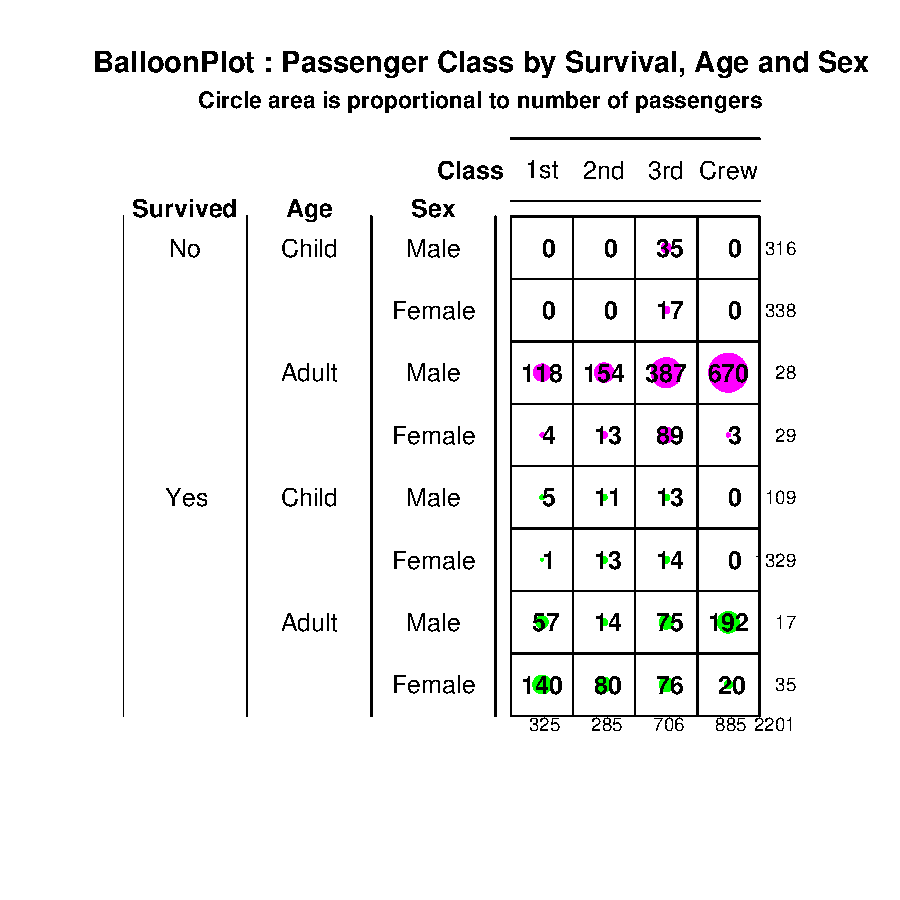
\includegraphics[width=\textwidth]{Figure3.pdf}
\caption{\label{figure:Figure3}
  Balloon plot of Titanic passengers by gender, age and class. Green
  circles represent passengers who survived and magenta circles
  represent the passengers who did not survive.}
\end{figure}

Figure~\ref{figure:Figure3} conveys much more information than
figures 1 and 2 without loss of clarity. Bigger circles of magenta
color make it clear that the number of passengers who did not
survive is significantly bigger than that of passengers who
survived.


Still, to make further improvements in the display, we redraw the
same data and add the cummulative sums accross each row and column,
 histograms across each section, and legend, as shown in figure 4.
  This is accomplished using the code:

{
\small
\begin{verbatim}

library(gplots)
data(Titanic)
dframe <- as.data.frame(Titanic) 
attach(dframe)
colors <- ifelse( Survived=="Yes", "green", "magenta")

balloonplot(x=Class, y=list(Survived, Age, Sex),
            z=Freq, sort=TRUE, dotcol=colors,
            show.zeros=TRUE, main="BalloonPlot :
            Passenger Class by Survival, Age and Sex")

title(main=list("Area is proportional to number of
            passengers", cex=0.9), line=0.5)

legend(3,0.5, legend=c("Not survived","Survived"),
       col=c("magenta","green"), pch=20, cex=.8,
       pt.cex=0.8, text.col=c("magenta", "green"),
       horiz=TRUE, xjust=0.5, bty="n")

\end{verbatim}
 }
%$

\begin{figure}
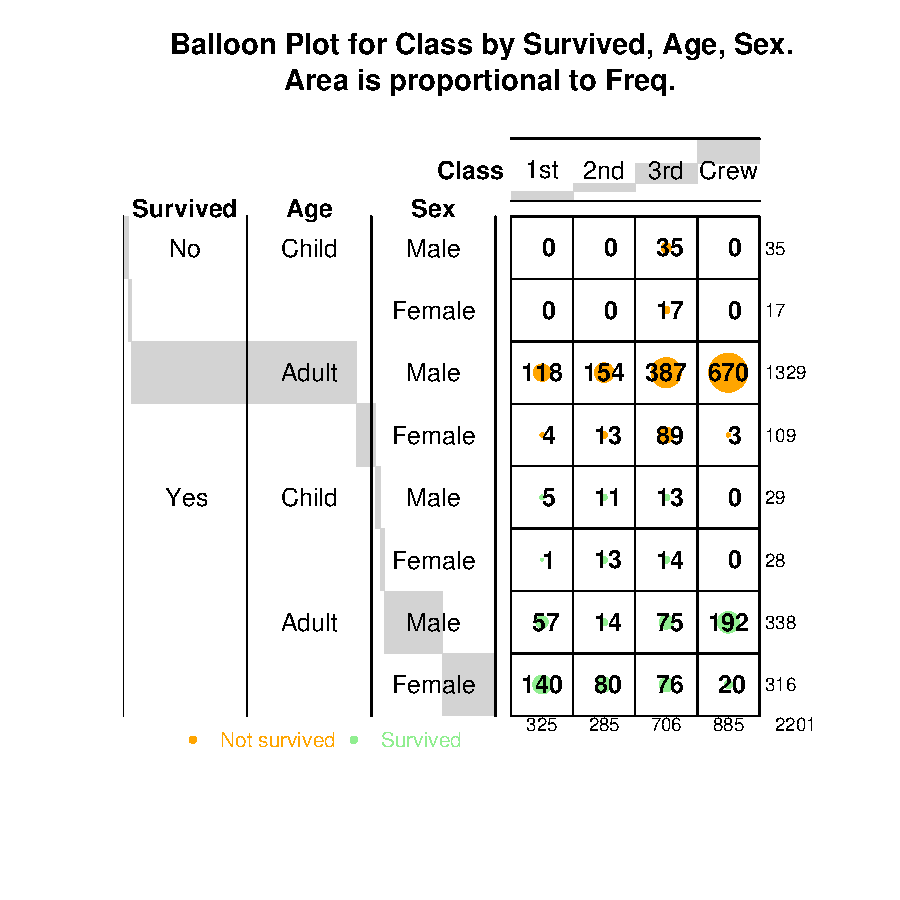
\includegraphics[width=\textwidth]{Figure4.pdf}
\caption{\label{figure:Figure4}
Balloon plot of all the passengers of Titanic, stratified by survival, age, sex
and class}
\end{figure}

It is now easy to see that adult females and adult male crew members
survived in large numbers. Figure~\ref{figure:Figure4} displays many
features of the Titanic passengers. Passengers who survived are
shown in green circles and passeengers who did not survive are shown
in magenta circles. Sums across rows and columns are represented in
the numbers at the right and bottom respectively.  The shaded
rectangular blocks show the density of data.  From the figure, it
can be clearly seen that the largest number of individuals who did
not survive are adult male crew (670). $1^{st}$ class adult females
were among the group of people who survived the most. Since there
were no child-crews and all the children survived, some fileds are
left empty in the figure. 





%%In order to investigate further,
%%let us examine the number of individuals belonging to each
%%category:
%%
%%\vspace{-0.25in}
%%
%%{\small
%%\begin{verbatim}
%%total.pop <- cbind(apply(Titanic[,,Age="Child",],
%%                         c(1,2), sum), 
%%                   apply(Titanic[,,Age="Adult",], 
%%                         c(1,2), sum))
%%colnames(total.pop) <- c("Child-M", "Child-F", 
%%                         "Adult-M", "Adult-F")
%%balloonplot(as.table(total.pop), xlab="",
%%            ylab="", main="")
%%title("BalloonPlot : Total passengers by
%% gender and age")
%%mtext("(Area proportional to frequency)")
%%\end{verbatim}
%% }
%%
%%
%%\begin{figure}
%%%\vspace*{.1in}
%%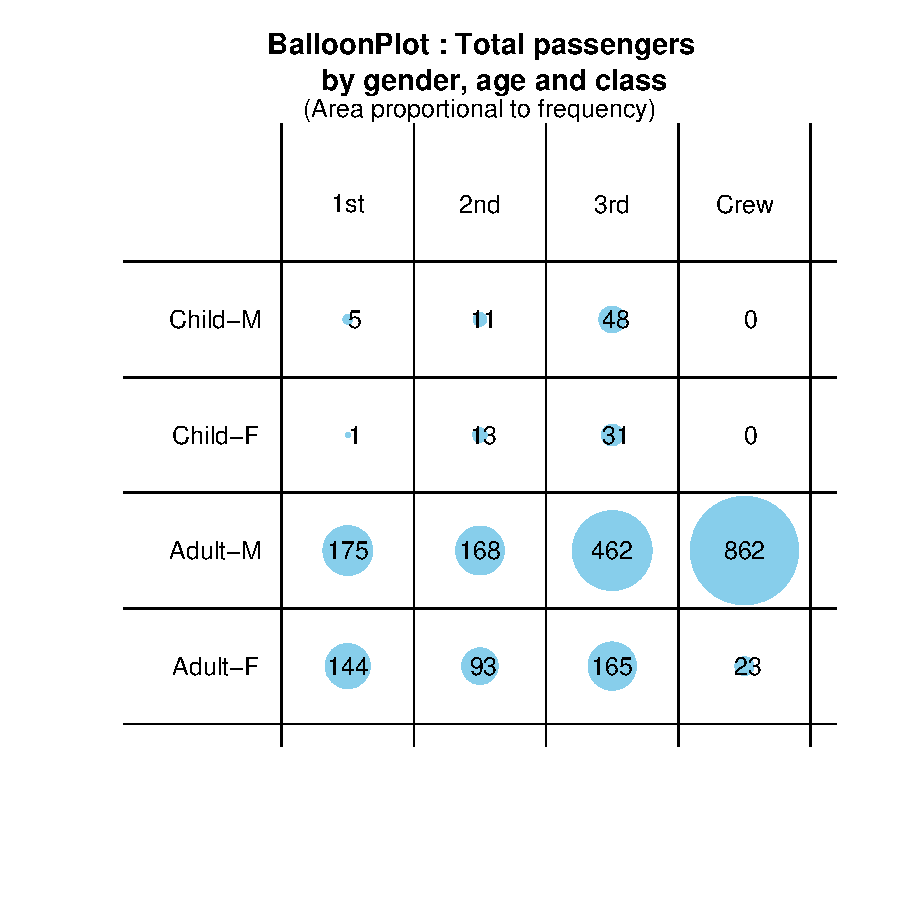
\includegraphics[width=\textwidth]{TotalPop.pdf}
%%\caption{\label{figure:Total.Pop}
%%Balloon plot of total population}
%%\end{figure}
%%



%% adult male crew (862), followed by adult males in
%%$3^{rd}$ class (462).  Thus it is not surprising that a large number of
%%adult male crew members survived.  However, we now see that survival
%%among $3^{rd}$ class adult males should have been high too.  So, let us
%%look at the fraction of passengers from each group who survived.
%%
%%{\small
%%\begin{verbatim}
%%
%%surv.prop <- as.table(surv.pop/total.pop)
%%
%%surv.prop[is.na(surv.prop)] <- 0
%%
%%balloonplot(as.table(surv.prop), xlab="",
%%            ylab="", main="")
%%title("BalloonPlot : Surviving passengers
%% by gender and age")
%%mtext("(Area proportional to frequency)")
%%\end{verbatim}
%%}
%%
%%
%%\begin{figure}
%%%\vspace*{0.1in}
%%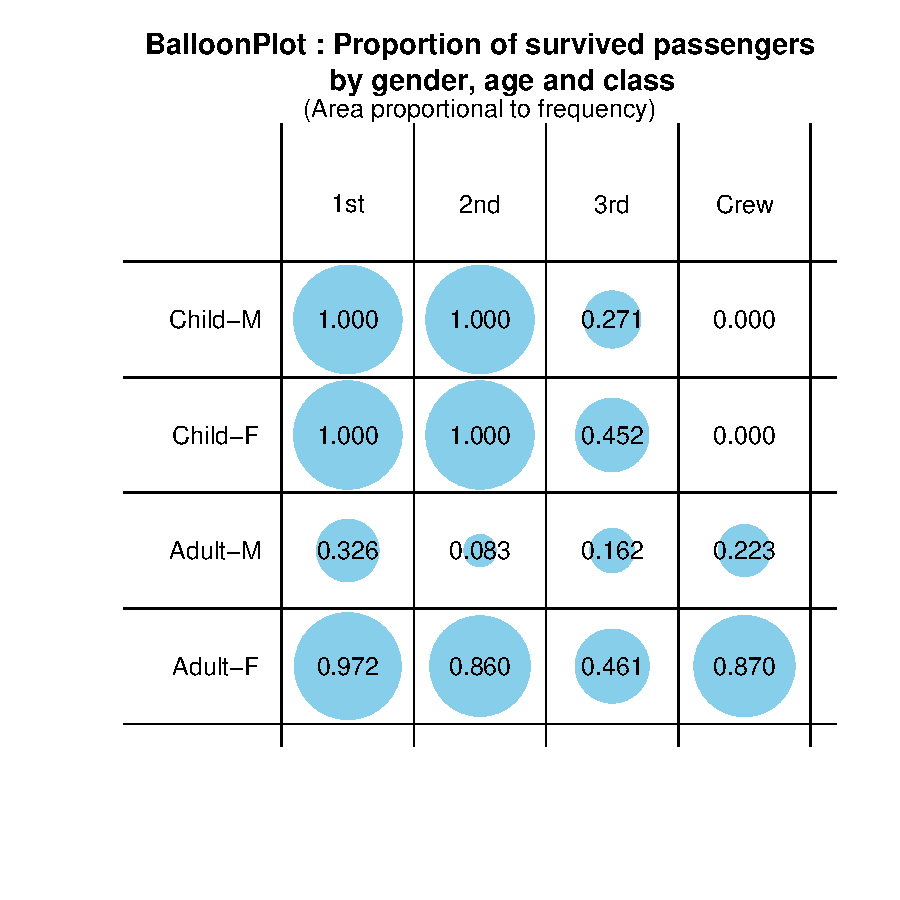
\includegraphics[width=\textwidth]{SurvivedProp.pdf}
%%\caption{\label{figure:Surv.Prop}
%%Balloon plot of proportion of people surviving}
%%\end{figure}
%%

%%Figure\ref{figure:Surv.Prop} shows a diferent aspect of data. We can
%%now easily see from size of the circles that all the children in
%%$1^{st}$ and $2^{nd}$ class survived, as did most of the women in
%%$1^{st}$ and $2^{nd}$ class as well as female crew.  It is now clear
%%that there is something distinctly different about survival among
%%$3^{rd}$ class passengers: it is much lower than survival in any of the
%%other classes.
%%
It turns out that there is a well known reason for this difference.
Passengers in $1^{st}$ and $2^{nd}$ class, as well as crew members, had an
easier time reaching the lifeboats.  Since there were too few
lifeboats for the number of passengers and crew, most women and
children among the first and second class passengers as well as
female crew found space in a lifeboat, while many of the later
arriving $3^{rd}$  class women and children were too late: the lifeboats
had already been filled and had moved away from the quickly sinking
ship.

\section*{Conclusion}

Using the well worn Titanic data, we have shown how balloonplots
help to convey important aspects of tabular data, without obscuring
the exact numeric values. We hope that this new approach to
visualizing tabular data will assist other statiticians in more
effectively understanding and presenting tabular data.

We wish to thank \emph{Ramon Alonso-Allende}
\email{allende@cnb.uam.es} for the discussion on R-help which lead
to the development of \code{balloonplot}. Ramon also added the code
to display the row- and column sums.

\address{Gregory R. Warnes, Pfizer Inc., USA\\
\email{gregory.r.warnes@pfizer.com}\\
       Nitin Jain, Pfizer Inc., USA\\
\email{nitin.jain@pfizer.com}}

\end{article}

\end{document}
